% Inicio del ApÈndice A
\chapter{Nombre del Apéndice}\label{apendiceA}

\section{Imágenes}
\begin{figure}[H]
\centering
         \begin{subfigure}{0.8\textwidth}
         \centering
         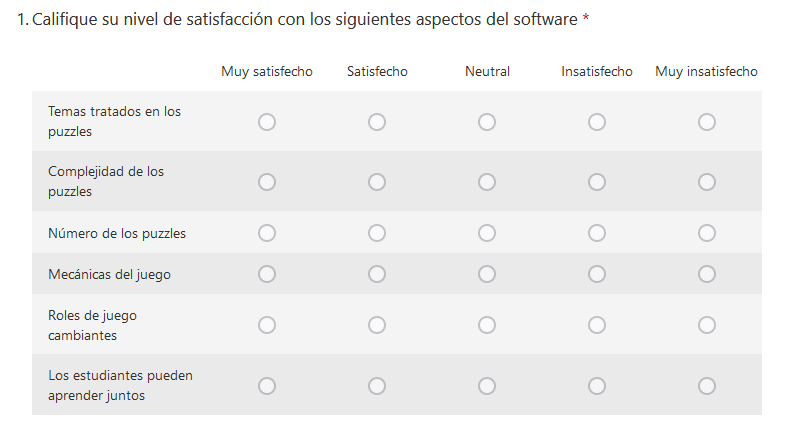
\includegraphics[width=\textwidth]{images/PreguntaEncuesta (4).png}
         \caption{Pregunta 1.}
         \label{fig:survey1}
    \end{subfigure}

        \begin{subfigure}{0.8\textwidth}
         \centering
         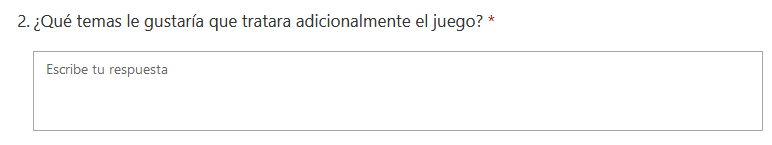
\includegraphics[width=\textwidth]{images/PreguntaEncuesta (5).png}
         \caption{Pregunta 2.}
         \label{fig:survery2}
     \end{subfigure}
\end{figure}
\begin{figure}
\ContinuedFloat
    \centering
    \begin{subfigure}{0.8\textwidth}
         \centering
         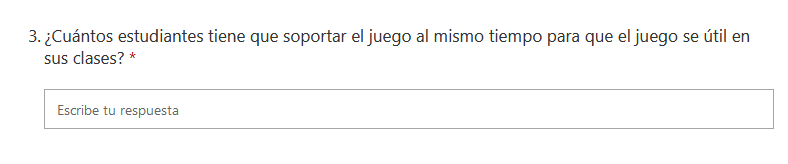
\includegraphics[width=\textwidth]{images/PreguntaEncuesta (1).png}
         \caption{Pregunta 3.}
         \label{fig:survey3}
    \end{subfigure}
    \begin{subfigure}{0.8\textwidth}
         \centering
         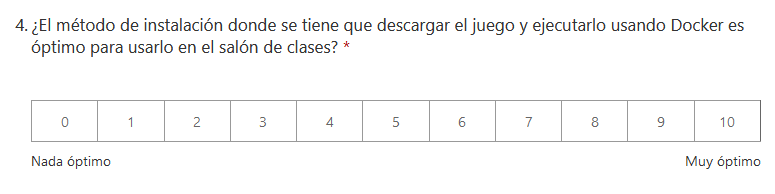
\includegraphics[width=\textwidth]{images/PreguntaEncuesta (2).png}
         \caption{Pregunta 4.}
         \label{fig:survery4}
     \end{subfigure}
    \begin{subfigure}{0.8\textwidth}
         \centering
         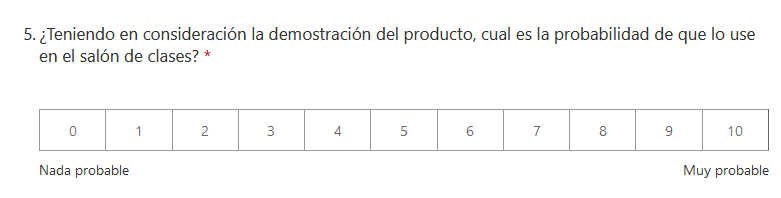
\includegraphics[width=\textwidth]{images/PreguntaEncuesta (3).png}
         \caption{Pregunta 5.}
         \label{fig:survery5}
    \end{subfigure}
        \caption{Preguntas de la encuesta a docentes respecto al juego.}
    \label{fig:survey}
\end{figure}

\section{Tablas}
\begin{longtable}[c]{ >{\centering\arraybackslash}p{2.75cm} >{\centering\arraybackslash}p{2.25cm} >{\centering\arraybackslash}p{2.25cm} >{\centering\arraybackslash}p{2.25cm} >{\centering\arraybackslash}p{2.25cm} >{\centering\arraybackslash}p{2.25cm}}
\caption{Resultados obtenidos de la encuesta a profesores\label{table:resultados_survey}.} \\
\linespread{0.5}\selectfont\centering
\setlength{\tabcolsep}{2pt}
\renewcommand{\arraystretch}{0.75}
         & Docente 1 & Docente 2 & Docente 3 & Docente 4 & Docente 5 \\ \hline
        Temas tratados en los puzzles & Neutral & Satisfecho & Satisfecho & Satisfecho & Satisfecho \\ \hline
        Complejidad de los puzzles & Neutral & Satisfecho & Satisfecho & Satisfecho & Satisfecho \\ \hline
        Número de puzzles & Neutral & Satisfecho & Neutral & Neutral & Neutral \\ \hline
        Mecánicas del juego & Insatisfecho & Satisfecho & Satisfecho & Muy satisfecho & Satisfecho \\ \hline
        Roles de juego cambiantes & Neutral & Neutral & Satisfecho & Muy satisfecho & Satisfecho \\ \hline
        Los estudiantes pueden aprender juntos & Muy satisfecho & Satisfecho & Satisfecho & Satisfecho & Muy satisfecho \\ \hline
        ¿Qué temas le gustaría que tratara adicionalmente el juego? & Temas acordes a la carta descriptiva & Arreglos y matrices & Arreglos y matrices. & Arreglos, matrices, código C básico. & Aumentar la complejidad, anexar arreglos y SubProcesos \\ \hline
        ¿Cuántos estudiantes tiene que soportar el juego al mismo tiempo para que el juego se útil en sus clases? & 30 & Sería bueno 30  & 30 & 20 mínimo & Mis grupos regularmente son de 40 estudiantes \\ \hline
        ¿El método de instalación donde se tiene que descargar el juego y ejecutarlo usando Docker es óptimo para usarlo en el salón de clases? & 7 & 10 & 7 & 8 & 9 \\ \hline
        ¿Teniendo en consideración la demostración del producto, cual es la probabilidad de que lo use en el salón de clases? & 5 & 8 & 7 & 10 & 9 \\ \hline
\end{longtable}